\chapter{Vorgehen}
In der Vorbereitung wurden schon früh die Werkzeuge für die Umsetzung und Konzeption gewählt, welche das Projekt strukturieren und planen sollten. Dabei kamen Mittel wie Kugelschreiber, Notizbücher, Kalender oder auch die Mindmap zum Einsatz. Mittels Requirement Engeneering wurde eine Anforderungsanalyse erstellt. Um einen übersichtlichen Workflow zu haben, fiel die Entscheidung Scrum als Vorgehensmodell für den künftigen Ablauf zu wählen.

\section{Versionsverwaltung}
Für die Versionsverwaltung wurde Git gewählt. Es handelt sich um ein Dezentrales Versionsverwaltungssystem und ist nicht von einem Bestimmten Server verbunden. In einem Versionsverwaltungssystem werden Verschiedene Entwicklungszustände gesichert. Damit ist es möglich zu sehen, wie sich eine Software entwickelt hat. Sollte ein Fehler auftreten, kann zu einer älteren Version gewechselt werden, in welcher der Fehler nicht vorhanden ist. Diese Versionen werden in einem Repository verwaltet.\autocite{git}



\section{Scrum}
\label{scrum}

Unter Scrum versteht man in der Projektplanung ein agiles Vorgehensmodell in der Softwareentwicklung. Es besteht aus mehreren Komponenten wie, Rollen Artefakte und Meetings. Sobald die Anforderungen und Eigenschaften eines Produktes angelegt worden sind, legt sie der Product Owner in einem sogenannten Product Backlog an. Daraufhin wird ein Sprint geplant. Es werden Anforderungen und Eigenschaften gewählt, welche in einem bestimmten Zeitraum erledigt werden können. Diese wiederum werden in das sogenannte Sprint Backlog abgelegt. Darauf erfolgt ein Sprint. Welcher nicht länger al ein Monat dauern sollte. Während des Sprints Tauscht sich das Entwicklerteam über den täglichen Status der Entwicklung aus. Man spricht von einem Daily Meeting. Jeder ist auf dem aktuellen Stand und es kann sofort eingegriffen werden, wenn es an einer Stelle zu Schwierigkeiten kommt. Ist ein Sprint abgeschlossen kann ein funktionierender Softwareteil präsentiert werden. \autocite{Niermann.2017}

\begin{figure}[H]
	\centering
	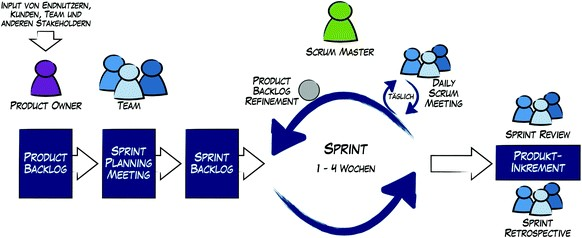
\includegraphics[scale=0.95]{content/pictures/scrum.jpg}
	% bosch_iot_poll.png: 0x0 pixel, 300dpi, 0.00x0.00 cm, bb=
	\caption{Ablauf eines Scrums. \cite{Niermann.2017}}
	\label{fig:scrum}
\end{figure}

\subsection{Scrum als Einzelperson}
In dieser Arbeit wurde alleine und nicht im Team gearbeitet. Auch wenn es hierdurch keine Rollenverteilung gab, so konnte Scrum doch ideal eingesetzt werden. Das Backlog wurde mit Hilfe der Konzeption erzeugt. Mit der Planung wurde klar, welche Anforderungen an die Software bestehen. Diese wurden alle handschriftlich in ein Productbacklog niedergeschrieben. Darauf wurde mit dem Betreuer besprochen, welche aufgaben innerhalb von zwei Wochen erledigt seien sollen und wurden, ebenfalls handschriftlich, in das Sprintbacklog aufgenommen. Während des Sprints sind die Daily Meetings entfallen, da diese nicht nötig waren. Als einzelne Person ist man immer über den aktuellen Stand seiner Entwicklung bewusst. Ein tägliches Austauschen mit Teammitglieder ist nicht nötig, da es kein Team gibt. Nach den vergangenen zwei Wochen, wurde der Aktuelle Stand in einem Protokoll dokumentiert. Erfolge und Probleme wurden im Anschluss mit dem Erstbetreuer und der Zweitbetreuerin besprochen. Daraufhin wurde, wenn es nötig wurde, das Productbacklog erweitert. Aus diesem  Backlog wurden erneut Aufgaben für den nächsten Sprint gewählt. Der Entwickler übernahm so alle Rollen, welche in dem Vorgehensmodell Scrum definiert sind.

